\documentclass{beamer}

\usepackage[utf8]{inputenc}
\usepackage{listings}
\usepackage{listings-rust}
\lstset{
  frame=tb,
  aboveskip=3mm,
  belowskip=3mm,
  showstringspaces=false,
  columns=flexible,
  basicstyle=\footnotesize\ttfamily,
  % basicstyle={\small\ttfamily},
  numbers=left,
  numbersep=5pt,
  % xleftmargin=\parindent,
  numberstyle=\color{gray},
  keywordstyle=\bfseries\color{blue},
  commentstyle=\color{dkgreen},
  stringstyle=\color{mauve},
  breaklines=true,
  breakatwhitespace=false,
  tabsize=2
}
\usepackage{tikz}
\usetikzlibrary{fit,positioning}
\definecolor{tumblue}{RGB}{0,101,189}
\definecolor{dkgreen}{rgb}{0,0.6,0}
\definecolor{mauve}{rgb}{0.58,0,0.82}
\definecolor{cgreen}{RGB}{60,201,65}
\setbeamerfont{footnote}{size=\tiny}
\renewcommand\footnoterule{}
\usecolortheme{orchid}
\setbeamertemplate{navigation symbols}{}
\setbeamertemplate{sidebar right}{% also implies no navbar
  \llap{\tikz\fill[tumblue,scale=.1] (0,0) ++(-5cm,-5cm) ++(-10cm,0)
      +(0cm,0cm) -- +(4cm,0cm) -- +(4cm,-4cm) -- +(5cm,-4cm) -- +(5cm,0cm) --
      +(10cm,0cm) -- +(10cm,-5cm) -- +(9cm,-5cm) -- +(9cm,-1cm) --
      +(8cm,-1cm) -- +(8cm,-5cm) -- +(7cm,-5cm) -- +(7cm,-1cm) --
      +(6cm,-1cm) -- +(6cm,-5cm) -- +(3cm,-5cm) -- +(3cm,-1cm) --
      +(2cm,-1cm) -- +(2cm,-5cm) -- +(1cm,-5cm) -- +(1cm,-1cm) --
      +(0cm,-1cm) -- cycle;}
  % Slide number in triangle.
  \vfill\llap{\tikz\path[fill=tumblue,inner sep=3pt] (0,0) -- ++(-1cm,0) -- +(1cm,1cm) -- cycle node[anchor=south east] {\usebeamerfont{footline}\color{white}\bfseries\insertframenumber};}%
  % Variant without triangle
  % \vfill\llap{\usebeamerfont{footline}\usebeamercolor[fg]{footline}\insertframenumber\hskip3pt}\vskip3pt%
}

\title{Ownership types in theory and practice (in Rust)}
\author{Fritz Rehde}
\institute{School of Computation, Information, and Technology\\Technical University of Munich}
\date{26.01.2023}


\begin{document}

\frame{\titlepage}

\begin{frame}{Overview}
\tableofcontents
\end{frame}

\section{Motivation}

\begin{frame}{Memory safety}
\begin{itemize}
  \item definition: program is memory safe if all memory pointers or references always refer to valid memory
  \item Google and Microsoft: 70 percent of vulnerabilities due to memory safety issues
  \item National Security Agency (USA) recommends memory-safe languages (instead of C/C++)
  \item examples: buffer overflows, memory leaks, double-free, use-after-free
  \item result: malicious exploits, incorrect program results, "random" crashes
\end{itemize}
\end{frame}


\begin{frame}{Aliasing}
\begin{itemize}
  \item object aliasing: accessing the same memory through different symbolic names
  % TODO: example
  \item how to prevent bugs through (unintentional) aliases $\rightarrow$ bugs (hard to detect)
  \begin{itemize}
    \item ban aliasing altogether?
    \item restrict where and how aliasing can be used (through ownership rules) $\rightarrow$ improve memory safety
  \end{itemize}
\end{itemize}
\end{frame}


\begin{frame}[fragile]{Aliasing: example}
C++
\begin{lstlisting}[language=C++]
std::vector<int> v { 10, 11 };
int *vptr = &v[1];  // points into v
v.push_back(12);    // v buffer reallocated => vptr dangling
std::cout << *vptr; // bug (use-after-free)
\end{lstlisting}

Rust
\begin{lstlisting}[language=Rust]
let mut v = vec![10, 11];
let vptr = &mut v[1];  // 1. mutable reference
Vec::push(&mut v, 12); // 2. mutable reference
println!("{}", *vptr); // compiler error
\end{lstlisting}

Observation: an action through an object (\emph{v}) will also affect all of its aliases (\emph{vptr}), even though these aliases might not "expect" a change.
\end{frame}


\section{Ownership types in theory}

\begin{frame}{Ownership types}
\begin{itemize}
  \item object-oriented programs:
  \begin{itemize}
    \item objects can reference any other object
    \item objects can read and modify other objects' fields
    \item makes it difficult to understand, to maintain, and to reason about
  \end{itemize}
  \item using ownership types:
  \begin{itemize}
    \item limit which objects can be referenced
    \item can specify whether the referenced objects may be mutated or just read from
  \end{itemize}
\end{itemize}
\end{frame}


\begin{frame}{Ownership types: core concepts}
\begin{itemize}
  % TODO: different highlighting than italics
  \item objects can be \emph{owners} of other objects
  \item \emph{inside} relation: \emph{a} is \emph{inside} \emph{b} if they are the same object or \emph{a} is transitively owned by \emph{b}
  \item \emph{outside} relation: converse of \emph{inside} relation
  \item \emph{ownership context}: set of all objects that an object owns
  \item \emph{siblings}: objects in the same ownership context
  \item special \emph{world} object is root of the ownership hierarchy tree
\end{itemize}

% TODO: make spacing between vertical objects smaller
\begin{figure}[fragile]
  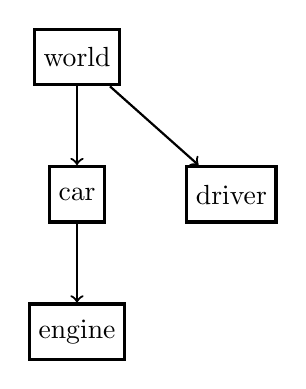
\begin{tikzpicture}[object/.style={rectangle, draw, very thick, minimum size=20}]
    \node[object] (World) {world};
    \node[object] (Car) [below=of World] {car};
    \node[object] (Driver) [right=of Car] {driver};
    \node[object] (Engine) [below=of Car] {engine};

    \draw[->,thick] (World) to (Car);
    \draw[->,thick] (World) to (Driver);
    \draw[->,thick] (Car) to (Engine);
  \end{tikzpicture}

  \caption{solid lines indicate "owns"}
\end{figure}
\end{frame}


\begin{frame}{Owners-as-dominators}
For \emph{a} to validly reference \emph{b}:
\begin{enumerate}
  \item \emph{a} is the owner of \emph{b},
  \item \emph{a} and \emph{b} are siblings, or
  \item \emph{b} is outside of \emph{a}.
\end{enumerate}

\begin{figure}[fragile]
  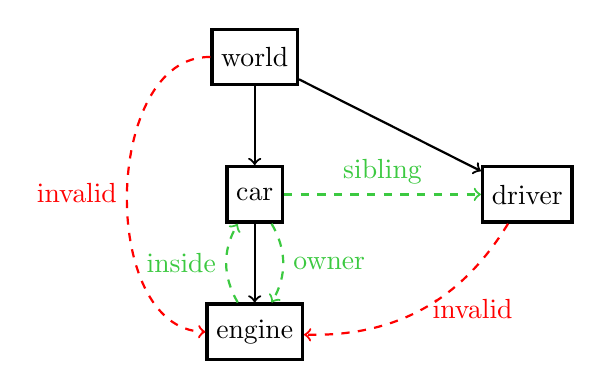
\begin{tikzpicture}[object/.style={rectangle, draw, very thick, minimum size=20}]
    \node[object] (World) {world};
    \node[object] (Car) [below=of World] {car};
    \node[object] (Driver) [right=of Car,xshift=1.5cm] {driver};
    \node[object] (Engine) [below=of Car] {engine};

    \draw[->,thick] (World) to (Car);
    \draw[->,thick] (World) to (Driver);
    \draw[->,thick] (Car) to (Engine);

    \draw[->,thick,dashed,cgreen] (Car) edge[bend left] node[right] {owner} (Engine);
    \draw[->,thick,dashed,cgreen] (Engine) edge[bend left] node[left] {inside} (Car);
    \draw[->,thick,dashed,cgreen] (Car) edge node[above] {sibling} (Driver);
    \draw[->,thick,dashed,red] (World) edge[bend right=90] node[left] {invalid} (Engine);
    \draw[->,thick,dashed,red] (Driver) edge[bend left] node[right] {invalid} (Engine);
  \end{tikzpicture}

  \caption{solid lines indicate "owns" and dotted lines indicate "references"}
\end{figure}
\end{frame}


\begin{frame}{Owners-as-dominators: implications}
\begin{itemize}
  \item any external reference to an object must go through its owner
  \item objects are only protected from external access, not internal access
  \item owners-as-dominators: owner is dominator for all of its owned objects
  \item doesn't allow common idioms that involve aliasing
  \item model restricts \emph{where} references can point, not \emph{how} references are used
\end{itemize}

\begin{figure}[fragile]
  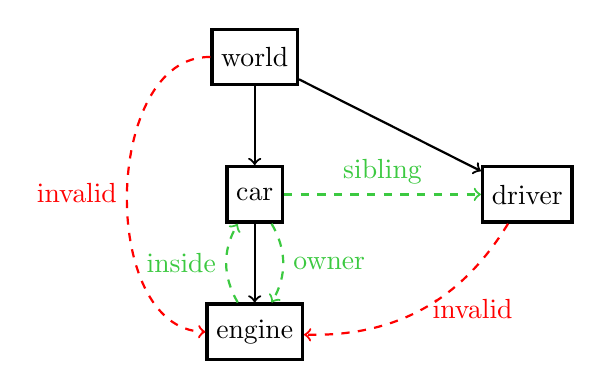
\begin{tikzpicture}[object/.style={rectangle, draw, very thick, minimum size=20}]
    \node[object] (World) {world};
    \node[object] (Car) [below=of World] {car};
    \node[object] (Driver) [right=of Car,xshift=1.5cm] {driver};
    \node[object] (Engine) [below=of Car] {engine};

    \draw[->,thick] (World) to (Car);
    \draw[->,thick] (World) to (Driver);
    \draw[->,thick] (Car) to (Engine);

    \draw[->,thick,dashed,cgreen] (Car) edge[bend left] node[right] {owner} (Engine);
    \draw[->,thick,dashed,cgreen] (Engine) edge[bend left] node[left] {inside} (Car);
    \draw[->,thick,dashed,cgreen] (Car) edge node[above] {sibling} (Driver);
    \draw[->,thick,dashed,red] (World) edge[bend right=90] node[left] {invalid} (Engine);
    \draw[->,thick,dashed,red] (Driver) edge[bend left] node[right] {invalid} (Engine);
  \end{tikzpicture}
\end{figure}
\end{frame}


\begin{frame}{Owners-as-modifiers}
Same rules as owners-as-dominators, but \emph{a} can also reference \emph{b} through \emph{r}, if:
\begin{enumerate}
  \item \emph{r} is a read-only reference and only pure methods (that don't modify existing objects) can be called on it.
\end{enumerate}

\begin{figure}
  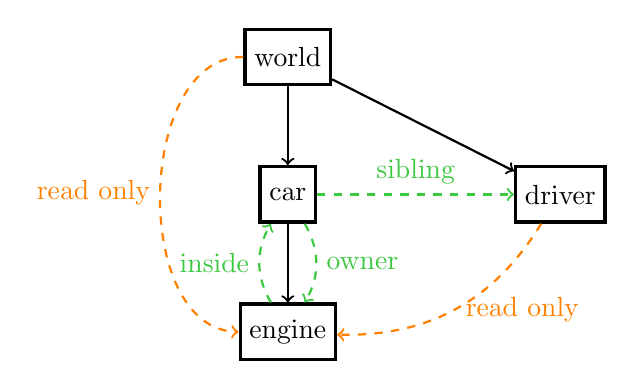
\begin{tikzpicture}[object/.style={rectangle, draw, very thick, minimum size=20}]
    \node[object] (World) {world};
    \node[object] (Car) [below=of World] {car};
    \node[object] (Driver) [right=of Car,xshift=1.5cm] {driver};
    \node[object] (Engine) [below=of Car] {engine};

    \draw[->,thick] (World) to (Car);
    \draw[->,thick] (World) to (Driver);
    \draw[->,thick] (Car) to (Engine);

    \draw[->,thick,dashed,cgreen] (Car) edge[bend left] node[right] {owner} (Engine);
    \draw[->,thick,dashed,cgreen] (Engine) edge[bend left] node[left] {inside} (Car);
    \draw[->,thick,dashed,cgreen] (Car) edge node[above] {sibling} (Driver);
    \draw[->,thick,dashed,orange] (World) edge[bend right=90] node[left] {read only} (Engine);
    \draw[->,thick,dashed,orange] (Driver) edge[bend left] node[right] {read only} (Engine);
  \end{tikzpicture}
\end{figure}
\end{frame}


\begin{frame}{Owners-as-modifiers: implications}
\begin{itemize}
  \item owners-as-modifiers: only the owners can modify objects
  \item model allows references to objects in arbitrary contexts, but restricts \emph{how} the references can be used
  \item fulfills requirements for verification of the functional correctness of object-oriented programs
\end{itemize}

\begin{figure}
  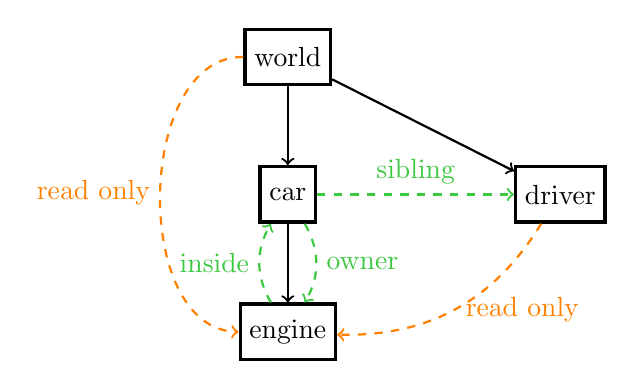
\begin{tikzpicture}[object/.style={rectangle, draw, very thick, minimum size=20}]
    \node[object] (World) {world};
    \node[object] (Car) [below=of World] {car};
    \node[object] (Driver) [right=of Car,xshift=1.5cm] {driver};
    \node[object] (Engine) [below=of Car] {engine};

    \draw[->,thick] (World) to (Car);
    \draw[->,thick] (World) to (Driver);
    \draw[->,thick] (Car) to (Engine);

    \draw[->,thick,dashed,cgreen] (Car) edge[bend left] node[right] {owner} (Engine);
    \draw[->,thick,dashed,cgreen] (Engine) edge[bend left] node[left] {inside} (Car);
    \draw[->,thick,dashed,cgreen] (Car) edge node[above] {sibling} (Driver);
    \draw[->,thick,dashed,orange] (World) edge[bend right=90] node[left] {read only} (Engine);
    \draw[->,thick,dashed,orange] (Driver) edge[bend left] node[right] {read only} (Engine);
  \end{tikzpicture}
\end{figure}
\end{frame}

\section{Ownership in Rust}

\begin{frame}{From theory to implementation}
\begin{itemize}
  \item Rust's ownership system: extends owners-as-modifiers
  \begin{itemize}
    \item no garbage collection (overhead)
    \item immutable (read-only) and mutable references % (not in owners-as-dominators)
    \item rules for compiler to check validity of references
    \item extensions:
    \begin{itemize}
      \item transferring ownership from one object to another
      \item object immutability by default
      \item Resource Acquisition Is Initialization (similar to C++)
    \end{itemize}
  \end{itemize}
  % \item aliasing concept essential to ownership types
  % \item different ways of implementing aliasing:
  % \begin{itemize}
  %   \item pointers: exist in Rust, but their use is not advised
  %   \item \emph{references}
  % \end{itemize}
  \item ownership rules in Rust:
  \begin{enumerate}
    \item Each value in Rust has an owner.
    \item There can only be one owner at a time.
    \item When the owner goes out of scope, the value will be \emph{dropped} (associated memory is freed).
  \end{enumerate}
\end{itemize}
\end{frame}


% \begin{frame}{Memory allocation system}
% \end{frame}

% TODO: variable scope


\begin{frame}[fragile]{Transferring ownership}
Heap-based values: 
\begin{itemize}
  \item unknown size at compile time
  \item copying the value at runtime could be costly
  \item values are "moved" (between variables) by default

  \begin{lstlisting}[language=Rust]
  fn main() {
    let a = String::from("hello world");
    let b = a; // ownership transfer: a is moved into b
    let c = take_ownership(b); // b is moved into function
    println!("{}", b); // compiler error: b no longer valid
  }
  fn take_ownership(s: String) -> String {
    // do something with s
    String::from("new hello world")
  }
  \end{lstlisting}
  \item create deep copies with explicit \verb|clone()| call
\end{itemize}
\end{frame}


\begin{frame}[fragile]{Transferring ownership}
Stack-based primitives: 
\begin{itemize}
  \item small, known size at compile time
  \item examples: i32, u8, f64, char, bool etc.
  \item values are copied by default

  \begin{lstlisting}[language=Rust]
  let x: u32 = 42;
  let y: u32 = x; // x is copied instead of moved
  println!("x: {}, y: {}", x, y); // x and y valid
  \end{lstlisting}
  \item stack-based values implement \verb|Copy| trait (exclusive to \verb|Drop| trait)
\end{itemize}
\end{frame}


\begin{frame}{Lifetimes}
\end{frame}


\begin{frame}{Borrowing}
\begin{itemize}
  \item \emph{reference}: an address that points to a value that is owned by another variable
  \item unlike \emph{pointers}, a reference is guaranteed to point to a valid value
  \item creating a reference in Rust is called \emph{borrowing}
  \item a reference does not own the value it points to $\rightarrow$ only reference (not the borrowed value) is dropped at the end of the reference's scope
  \item used for performing operations on values without taking ownership
  % \item the scope of a reference starts where it is introduced and extends until the last time it is used
  \item Rust supports immutable and mutable references
\end{itemize}
\end{frame}


\begin{frame}[fragile]{Borrowing: immutable references}
\begin{itemize}
  \item read-only/shared references $\rightarrow$ compiler disallows modifying borrowed value
  \item acquired using the \verb|&| operator
  \item unlimited amount of immutable references to same value are allowed (if no mutable references)

  \begin{lstlisting}[language=Rust]
  let s = String::from("hello");
  let r1 = &s; // 1. reference
  let r2 = &s; // 2. reference
  println!("r1: {}, r2: {}", *r1, *r2);
  \end{lstlisting}
\end{itemize}
\end{frame}


% TODO: combine this and next slide
\begin{frame}[fragile]{Borrowing: mutable references}
\begin{itemize}
  \item borrowed value may be modified
  \item acquired using the \verb|&mut| keyword
  \item borrowed value must be mutable with \verb|mut| (variables are immutable by default)

  \begin{lstlisting}[language=Rust]
  let mut s = String::from("hello");
  s.push_str(" world");
  String::push_str(&mut s, " world"); // equivalent
  \end{lstlisting}
\end{itemize}
\end{frame}


\begin{frame}[fragile]{Borrowing: mutable references}
\begin{itemize}
  \item \emph{data races}: multiple pointers access the same data simultaneously and at least one is writing to the data
  \item goal: prevent \emph{data races} at compile time
    % TODO: latex beamer make stand out/highlight
  \item lifetime of mutable reference may not overlap with lifetime of any other (immutable or mutable) reference
  \item only one mutable reference to a value allowed at any given time
\end{itemize}
\end{frame}


\begin{frame}[fragile]{References and borrowing: examples}
\begin{itemize}
  \begin{lstlisting}[language=Rust]
  let a;
  {
    let b: u32 = 42;
    a = &b;
  }
  println!("{}", *a) // dereference a
  \end{lstlisting}

  \item Will it compile? \pause No.
  % TODO: lifetime explanation
  \item Why not? \pause Borrowed value 'b' does not live long enough/is used after being dropped.
  \item Refactored version that compiles:\pause

  \begin{lstlisting}[language=Rust]
  let a;
  let b: u32 = 42;
  a = &b;
  println!("{}", *a) // dereference a
  \end{lstlisting}
\end{itemize}
\end{frame}

% TODO: will it compile: create multiple mutable references, but only use one
% However, the following code example \cite{rust-book} shows that it is important to note that the creation of multiple mutable and immutable references with scopes that do not overlap is allowed.

%   \begin{lstlisting}[language=Rust]
%   let mut s = String::from("hello");

%   let r1 = &s; // allowed
%   let r2 = &s; // allowed
%   println!("{} and {}", r1, r2);

%   let r3 = &mut s; // allowed
%   r3.push_str(" world");
%   println!("{}", r3);
%   \end{lstlisting}

% Since \emph{r1} and \emph{r2} are not used after line 5, that is where their scopes end.
% The scope of the mutable reference \emph{r3} only starts in line 7.
% Therefore, the scopes of the mutable reference and the two immutable references do not overlap, and the program compiles.


\section{Evaluation: another implementation}



\section{Conclusions and outlook}

\begin{frame}{Conclusions and outlook}
  Here are some conclusions.
\end{frame}


\end{document}
